\documentclass[tikz]{standalone}

\usepackage{xcolor}

% Farbdefinitionen im HEX-Format
\definecolor{BgBase}{HTML}{0B131E}
\definecolor{BgPanel}{HTML}{111D2B}
\definecolor{TextSec}{HTML}{517C96}
\definecolor{AccPrim}{HTML}{00E5FF}
\definecolor{StatSucc}{HTML}{00FF66}
\definecolor{StatCrit}{HTML}{FF2A40}

\begin{document}

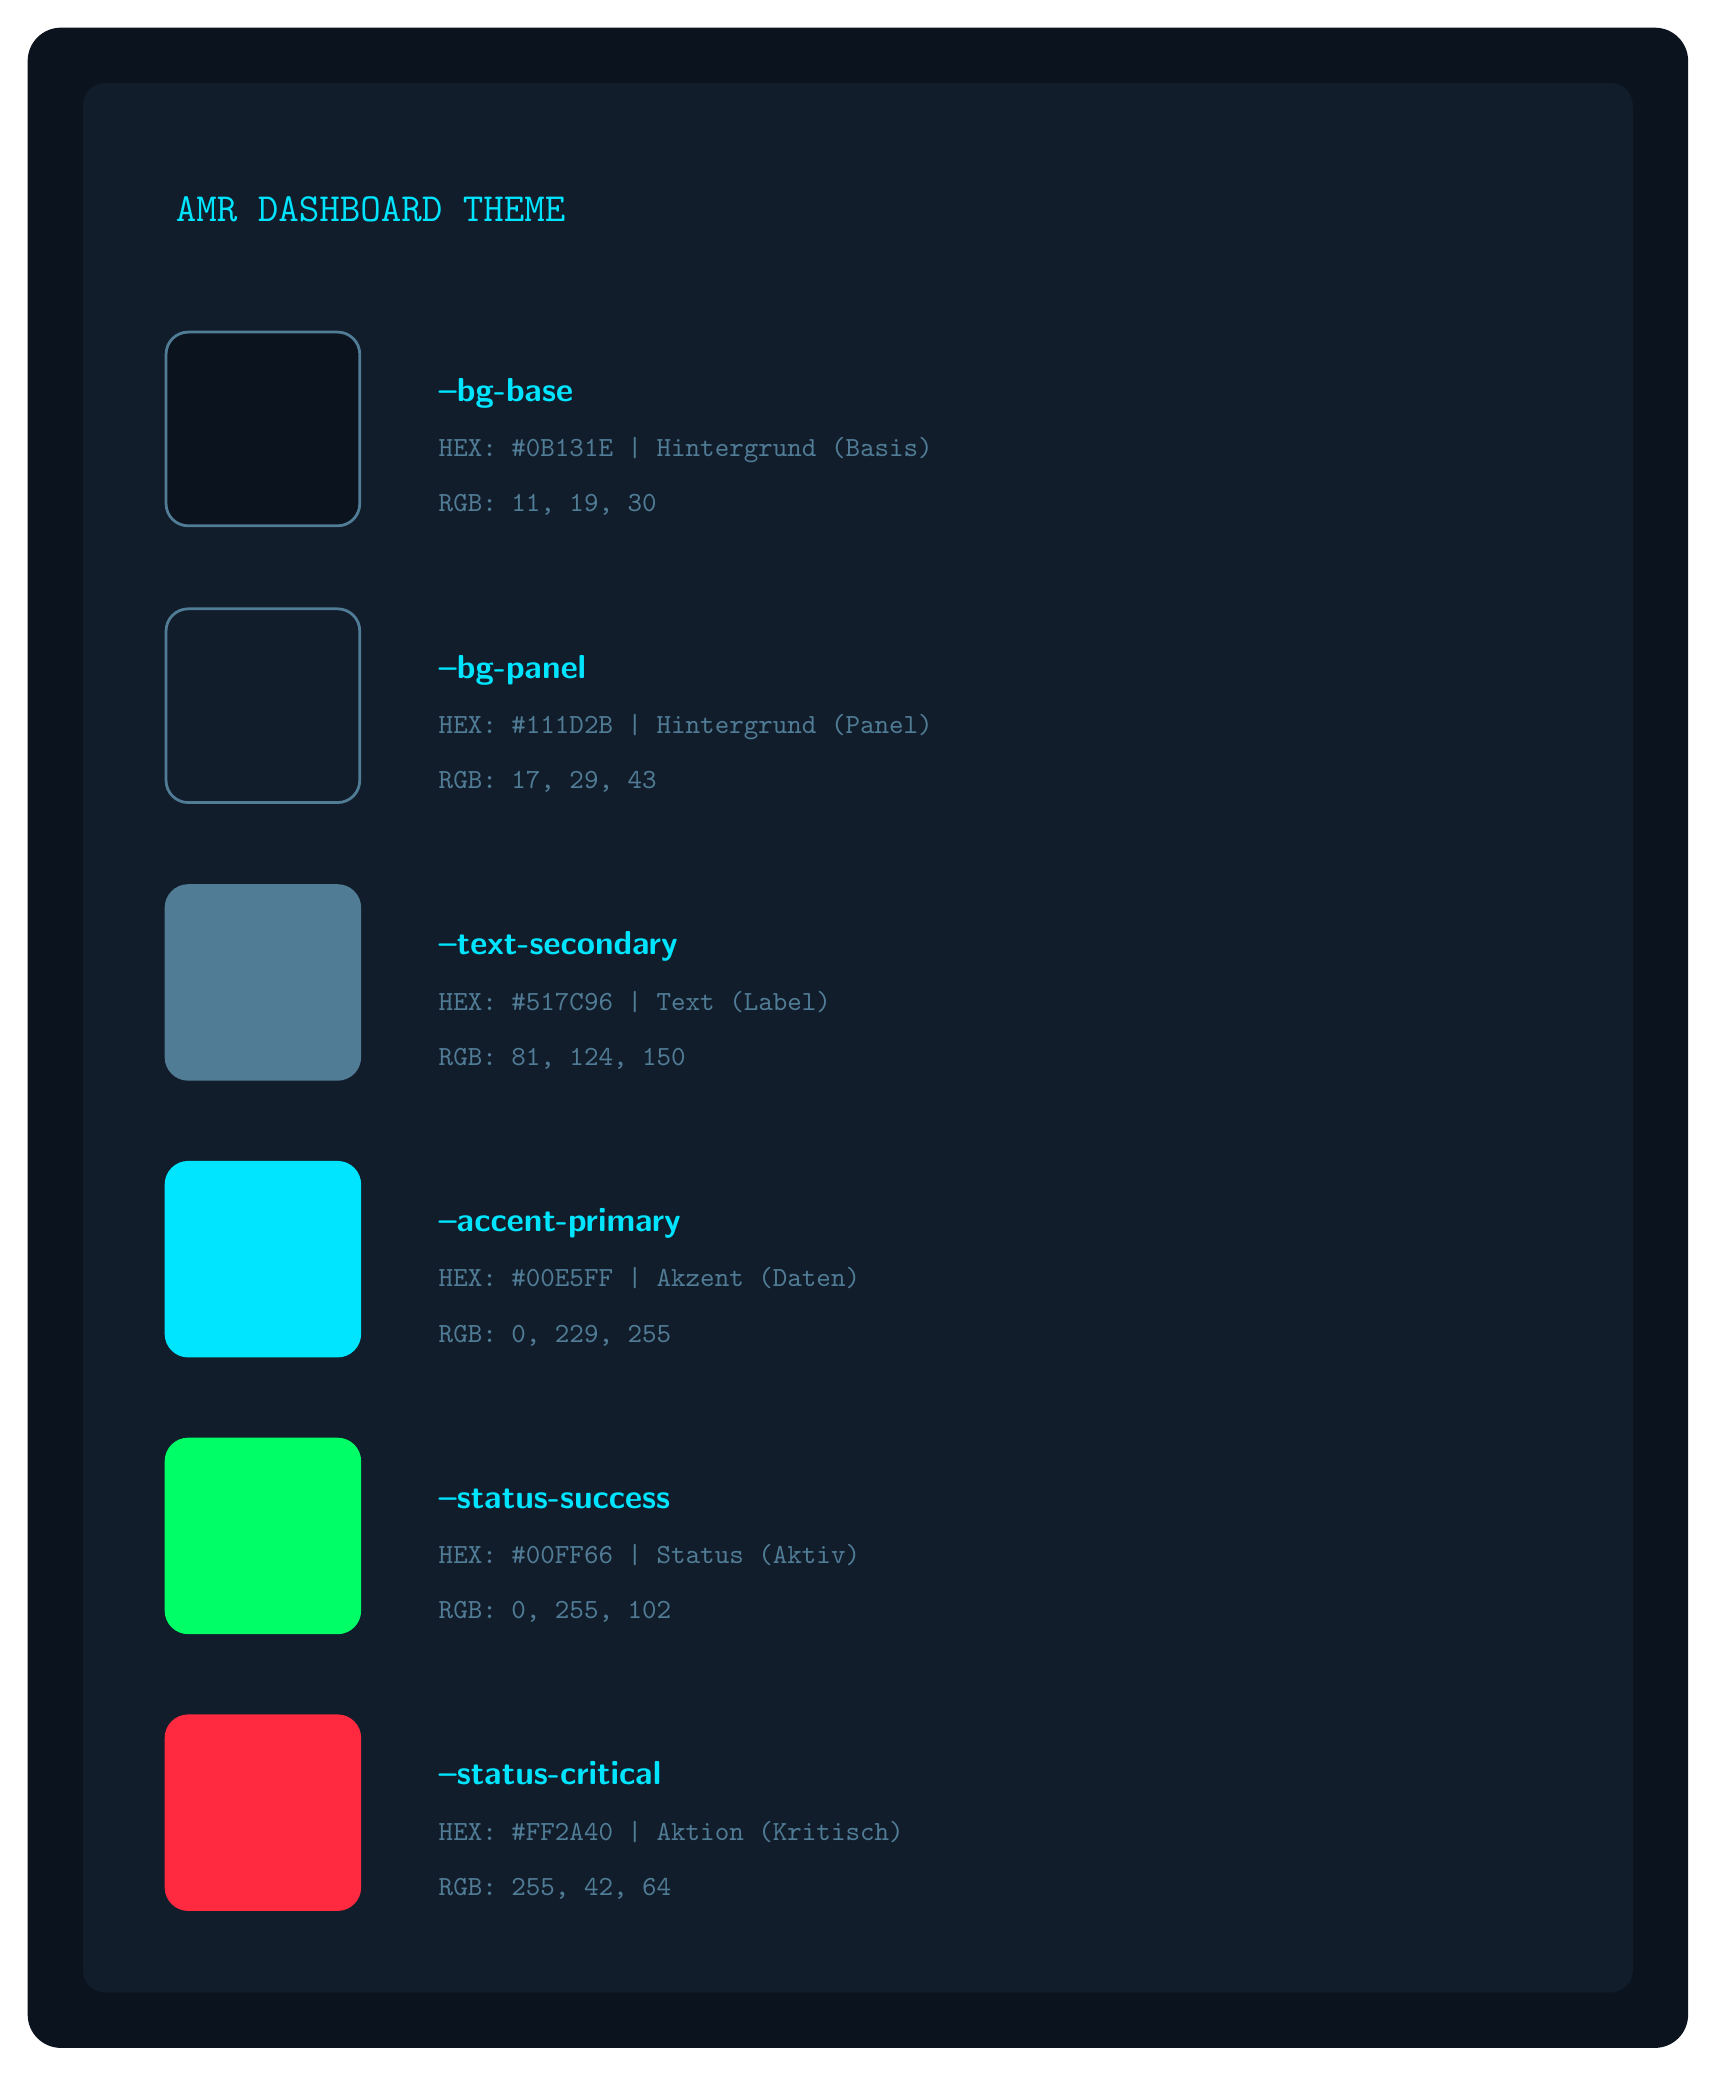
\begin{tikzpicture}[x=1pt, y=-1pt]

  % Container-Hintergründe
  \fill[BgBase, rounded corners=12pt] (0,0) rectangle (600,730);
  \fill[BgPanel, rounded corners=8pt] (20,20) rectangle (580,710);

  % Titel
  \node[anchor=base west, text=AccPrim, font=\ttfamily\bfseries\Large] at (50,70) {AMR DASHBOARD THEME};

  % Makro für einheitliche Farbfelder
  % Parameter: 1=y-Offset, 2=Fill, 3=Stroke, 4=Var-Name, 5=Hex-Text, 6=RGB-Text
  \def\paletteentry#1#2#3#4#5#6{
    \begin{scope}[shift={(50,#1)}]
      \filldraw[fill=#2, draw=#3, line width=1pt, rounded corners=8pt] (0,0) rectangle (70,70);
      \node[anchor=base west, text=AccPrim, font=\sffamily\bfseries\large] at (95,25) {#4};
      \node[anchor=base west, text=TextSec, font=\ttfamily] at (95,45) {#5};
      \node[anchor=base west, text=TextSec, font=\ttfamily] at (95,65) {#6};
    \end{scope}
  }

  % Rendering der Paletten-Einträge
  \paletteentry{110}{BgBase}{TextSec}{--bg-base}{HEX: \#0B131E | Hintergrund (Basis)}{RGB: 11, 19, 30}
  \paletteentry{210}{BgPanel}{TextSec}{--bg-panel}{HEX: \#111D2B | Hintergrund (Panel)}{RGB: 17, 29, 43}
  \paletteentry{310}{TextSec}{TextSec}{--text-secondary}{HEX: \#517C96 | Text (Label)}{RGB: 81, 124, 150}

  % Leuchtende Akzentfarben nutzen dieselbe Farbe für Fill und Stroke
  \paletteentry{410}{AccPrim}{AccPrim}{--accent-primary}{HEX: \#00E5FF | Akzent (Daten)}{RGB: 0, 229, 255}
  \paletteentry{510}{StatSucc}{StatSucc}{--status-success}{HEX: \#00FF66 | Status (Aktiv)}{RGB: 0, 255, 102}
  \paletteentry{610}{StatCrit}{StatCrit}{--status-critical}{HEX: \#FF2A40 | Aktion (Kritisch)}{RGB: 255, 42, 64}

\end{tikzpicture}

\end{document}
